\clearpage
\newpage

\section{Availability Estimation}
\label{sec-model}

In order for parking events to be useful, they must be incorporated into a
model allowing us to predict parking lot availability. Our goal is to respond
to queries with the probability that a given parking has a space available,
information that can be used in several ways to determine what lots to search
and in what order. PocketParker's estimator uses the events produced by our
parking event detector both to estimate the rates at which drivers are
searching and departing from the lot and to adjust the availability
probability directly. In this section, we present the design of the
PocketParker parking lot availability estimator and portions of our system
that run on the backend server.

\subsection{Overview}

\begin{figure}
\centering
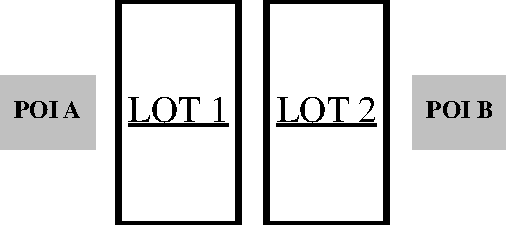
\includegraphics[width=\columnwidth]{./figures/CartoonLot.pdf}

\caption{\textbf{Example parking lot setup.} Two lots and three
destinations are shown.}

\label{fig-lots}
\end{figure}

Figure~\ref{fig-lots} shows an example setup with two parking lots and two
destinations used throughout this section. For each lot $l$, PocketParker
maintains a time-varying probability that the lot has $n$ free spots $P_l(t,
n)$. While we are mainly interested in the probability that the lot has a
space available $P_l(t, X > 0)$, we maintain separate probabilities for each
number of free spots so that we can manipulate individual probabilities in
response to events and queries as described below. We bound the count
probability distribution to lie between 0 and the capacity of the parking
lot. Section~\ref{subsec-capacity} briefly describes how PocketParker
estimates lot capacity.

PocketParker's estimator receives two types of events: arrivals and
departures. However, for each arrival in a given lot, a number of additional
lots may have been searched unsuccessfully, information critical to the
accuracy of our availability model. Section~\ref{subsec-lots} describes how
PocketParker determines relationships between parking lots, and
Section~\ref{subsec-implicit} describes how we combine that information with
arrivals to estimate implicit search behavior.

Between events we want to maintain our availability model by estimating the
rate at which departures and searches are taking place. PocketParker must use
the events it can detect to estimate the rate at which events are taking
place in the lot, which includes the effect of drivers not using
PocketParker, which we call \textit{hidden drivers}. Accomplishing this
requires that we estimate the ratio between monitored and hidden drivers, and
we describe an approach to doing so in Section~\ref{subsec-hidden}. With an
estimate of the hidden driver ratio, we can scale the search and departure
rates according, described in Section~\ref{subsec-rates}. Finally,
Section~\ref{subsec-online} describes how we integrate all of this
information to update our availability estimate as arrival and departure
events are received.

\subsection{Estimating Lot Capacity}
\label{subsec-capacity}

PocketParker requires an estimate of lot capacity $C$ in several places.
First, we use this estimate to bound $P_l(t)$ such that $P_l(t, X > C) =
0\;\forall\;t$. Second, we use the capacity to determine the number of hidden
drivers, explained in more detail in Section~\ref{subsec-hidden}.

Recall from Section~\ref{FIXME} that our false-positive filter uses knowledge
of the location of lots obtained from the OpenStreetMap database. We estimate
the capacity of each lot by converting the location of the lot into a size
and dividing by the size of an average parking spot. We use the parking lot design
standards provided in \cite{parkingdesign} to estimate the number of spots after estimating the 
area of the parking lot from which we detect an park event. \ref{} Shows our estimation accuracy 
for five lots in our campus.XXXnote \XXXnote{Anand and
Taeyeon, add capacity estimation stuff here. What is the size of the spot
that we determined? Reference for that. Estimates for each of the lots we
used and comparison with the true counts.} Errors in the capacity can result
if the size of parking spots in the lot differ from our estimate, or if the
parking lot is not efficiently packet with spots. Given the incentive of
parking lot designers to maximize capacity, we believe that the second case
will be unlikely. Parking spot sizes, however, may vary significantly from
lot to lot or based on the lot's location. To improve our estimate, we may
need to incorporate location-specific parking spot size estimates.
Alternatively, mapping databases may be directly annotated with the number of
spots per lot.

\subsection{Lot Relationships}
\label{subsec-lots}

PocketParker's detector identifies only arrivals and departures. However,
understanding and incorporating search behavior is critical to our model. For
example, if we observe the arrival rate fall at a given lot, it may be
because the lot is full, or it may be simply because fewer drivers are
arriving and the lot still has many spaces available.

In order to estimate search behavior, we need to understand the relationships
between parking lots. This requires two additional pieces of data about each
lot: one or multiple destinations, and a desirability index. The destination
represents the place the user is going when they park in a given lot, and
note that some lots may be associated with multiple destinations. In
Figure~\ref{fig-lots}, lot~1 may be associated with destinations A, B and C;
while lot~2 is only linked to B.

The desirability index produces an ordering of lots associated with a given
point-of-interest based on how preferable they are compared with other lots.
We assume that most users will park in desirable lots if they are available,
and may have searched in more desirable lots before parking in a lot
desirable lot. In Figure~\ref{fig-lots}, if Lot~2 is associated with
destination~A it will probably receive a lower desirability score than Lot~1
because it is further away.

While this information is not currently part of open mapping databases, we
believe that it is straightforward to collect. Parking lot operators and
business owners can annotate the mapping database with destinations for each
lot. In addition, data from navigation tools may be able to automatically
link destinations with lots by noting where users park after requesting
directions to a particular place. The desirability index may also be
determined by navigation tools observing what lots are searched by users on
their way to a particular destination. Lacking these traces, simple proximity
to the destination may determine the desirability index directly. As example
of this automatic annotation, in Figure~\ref{fig-lots} if both lot~1~and~2 are
associated with destination~A, we can consider lot~2 less desirable than
lot~1 because lot~1 lies between it and the destination.

\subsection{Implicit Searches}
\label{subsec-implicit}

With an understanding of lot relationships we can use observed arrivals to
model implicit---or unobserved---searches. When a user parks in a given lot,
we use the desirability index of the lot to add unsuccessful searches in more
desirable lots associated with the some destination. There are two challenges
to this approach. First, as described above, lots may be associated with
multiple destinations. Second, the user may not have actually performed the
search. After discussing both of these issues below,
Section~\ref{subsec-online} describe below how PocketParker incorporates the
information from implicit searches in a way sensitive to these uncertainties.

\subsubsection{Determining the destination}

If a lot is associated with multiple destinations, we cannot uniquely
determine the destination of the user. However, this only becomes important
if the two destinations would produce different desirability rankings for
affected lots. For example, in Figure~\ref{fig-lots}, if lots 1~and~2 are
both associated with destinations A~and~C, but not with B, then an arrival
with an unknown destination into lot~2 can always be used to generate an
implicit search in lot~1, since the desirability ranking for the two lots are
unchanged if the destination is either A~or~C. However, if both lots~1~and~2
are associated with all three destinations, then an arrival detected in lot~2
becomes more ambiguous. If the user was trying to go to destination~A, it may
mean that lot~1 was searched and is full; however, if they were trying to go
to destination~B, it may not indicate anything about lot~1. 

If lot destination annotations are generated by mapping software, we can use
this data to estimate the probability that a user is going to each of the
destinations associated with a particular lot. Instead of generating a single
implicit search in one lot, we generate multiple implicit searches in each of
the lots weighted by the destination probabilities. Lacking this arrival
data, we simply generate implicit searches in each destination associated
with a given lot.

\subsubsection{Speculative searches}

If we do not directly observe a user searching a lot before we detect an
arrival, we cannot be certain that they performed the search. If the
unsearched but preferable lot was available, they may not have searched it
because they prefer to choose the first available spot, enjoy the exercise of
walking farther to their destination, or want to irritate their passengers.
However, these are not the type of users we believe would benefit from or use
our PocketParker application, since finding a non-optimal parking spot is
fairly simple in most cases.

A more interesting case is where a user has not performed a search before
parking in a less-desirable lot because they \textit{believe} the more
desirable lot to be full. Users that park regularly at the same destination
usually have their own mental models for the availability of spots in certain
lots, causing them to discard those lots without searching them if they
believe the probability of finding a spot in the desirable lot is low. While
this behavior can cause users to miss available spots, these speculative
searches are useful inputs into our PocketParker model since it represents
what lots users think are full.

A final corner case that PocketParker does not handle is if all of the lots
for a given destination are full, and many undetected unsuccessful searches
are taking place. On one hand, if all lots are full then the availability of
spots is determined by departures, not arrivals, and so search data is
useless anyway. On the other hand, we would still like to identify this
situation for users that would prefer to avoid destinations where it is
difficult to park. While discussing future work in Section~\ref{sec-future},
we point out how integrating PocketParker into existing navigation
applications could address this problem by making searches explicit, rather
than implicit.

\subsection{Hidden Driver Estimation}
\label{subsec-hidden}

Monitored PocketParker users compete for parking spaces with unmonitored
users, which we call \textit{hidden drivers}. While we assume that
PocketParker users are generally representative of the entire driving
population, we do not assume that all or even a large fraction of drivers
will download and install PocketParker and we want our system to still
provide accurate predictions with the limited information caused by hidden
drivers. To accomplish this, PocketParker needs to estimate percentage of
drivers that are monitored, which we call the \textit{monitored fraction}. A
low monitored fraction indicates that few users are using PocketParker,
whereas a high monitored fraction means that we are receiving inputs from
most drivers. Put another way, the amount of uncertainty PocketParker must
face when predicting lot availability is inversely-proportional to the
monitored fraction.

\subsubsection{Importance of monitored fraction estimation}

Two examples will illustrate why we need this information and how it is used.
First, when a monitored driver leaves a parking lot, the monitored fraction
determines how long PocketParker will predict that a spot in that lot is
available. As the monitored fraction increases, the probability of
PocketParker seeing the arrival into the lot that occupies that spot
increases, and we can increase the amount of time that we estimate a spot is
available. On the other hand, as the monitored fraction decreases we see
fewer arrivals and are faced with more uncertainty. Hence, PocketParker
reduces the amount of time it predicts the spot is available. In
Section~\ref{subsec-online} we describe how hidden drivers influence the
changes to the availability model made when arrivals and departures are
detected.

Second, PocketParker uses the arrival and departure rates of monitored
drivers to estimate changes to parking lot availability over time. Here we
must scale the observed number of events to the actual number of events,
which requires an estimate of the monitored fraction.
Section~\ref{subsec-rates} describes how the monitored rate is used as an
input into rate estimation and scaling.

\subsubsection{Estimating the monitored fraction}
\label{subsubsec-monitored}

\begin{figure}
\centering
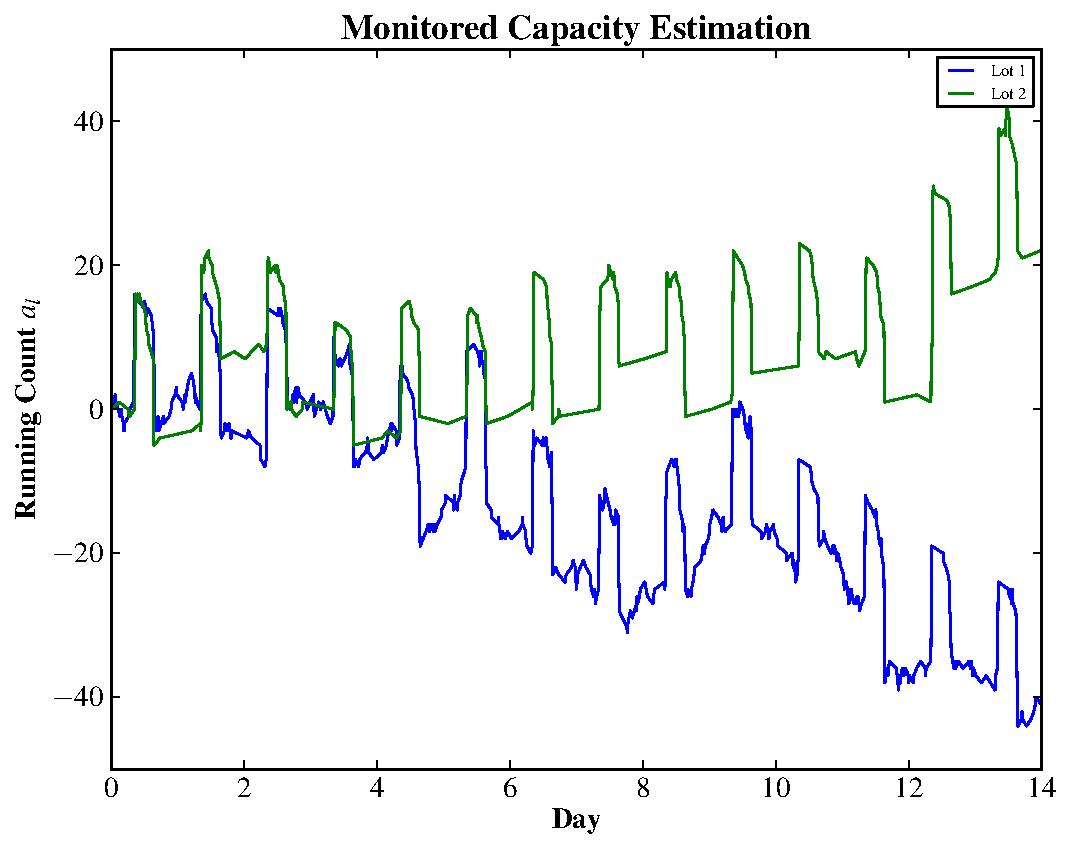
\includegraphics[width=\columnwidth]{./simulator/figures/capacity.pdf}

\caption{\textbf{Example of capacity estimation.} Running counts for two lots
are shown.}

\label{fig-capacityexample}
\end{figure}

PocketParker estimates the monitored fraction by first determining the
monitored capacity---the capacity of the lot measured by monitored
drivers---and then using our estimate of the lot capacity discussed in
Section~\ref{subsec-capacity}. Specifically, given a lot with capacity $C$,
the monitored fraction can be estimated as $f_m = \frac{C_m}{C}$. Our task
then becomes estimating the monitored capacity $C_m$.

To estimate the monitored capacity we maintain a running count $a_l$ for each
lot. When a monitored driver arrives in the lot, we decrement $a_l$; when a
monitored driver leaves the lot, we increment $a_l$. We can consider $a_l$ as
a estimate of the number of spots available in the lot scaled by $f_m$,
although we do not bound $a_l$ to be below the lot capacity or greater than
zero.

Figure~\ref{fig-capacityexample} shows an example of the running count for
two related lots over seven days using data generated by our lot simulator
described in Section~\ref{FIXME}. Both lots have capacity 200 and the actual
monitored fraction is 0.1. As the data shows, the running count experiences
long-period (greater than one day) fluctuations due to events missed by our
event detector and the randomness associated with the small percentage of
drivers being monitored. However, the data also contains short-period (less
than one day) fluctuations caused by the dynamics of the lot being monitored,
and these fluctuations are roughly the size of the monitored capacity $C_m$,
which in this case is 20 spots.

This observation motivates the design of our monitored capacity estimator.
First, we bin the data into 24~hour intervals. Next, we identify the largest
availability swing over each window. Finally, we average multiple swings
together for a period of days to determine the final estimate. This simple
approach works well on lots that fill on a regular basis. For the example in
Figure~\ref{fig-capacityexample}, our estimator estimates the monitored
capacity of lots~1~and~2 as 21.01 and 21.08, respectively, within 10\% of the
true value in both cases.We perform a further evaluation of our capacity
estimator using multiple lot simulations in Section~\ref{sec-evaluation}.

For lots that do not fill, or do not fill regularly, we may need to produce a
weighted sum where larger swings are weighted more heavily given our
assumption that they more accurately measure the true monitored capacity of
the lot. Another approach is to use the monitored fraction estimated at
desirable lots for a given destination, which are more likely to fill
completely and often, to estimate the monitored fraction for other
less-desirable lots. Here we are making the reasonable assumption that lots
connected to the same destination share similar fractions of PocketParker
users. Finally, PocketParker's monitored fraction estimator runs periodically
over up to a week's worth of data for each lot, to incorporate changes in the
monitored fraction caused by increasing use of our app.

\begin{figure}
\centering
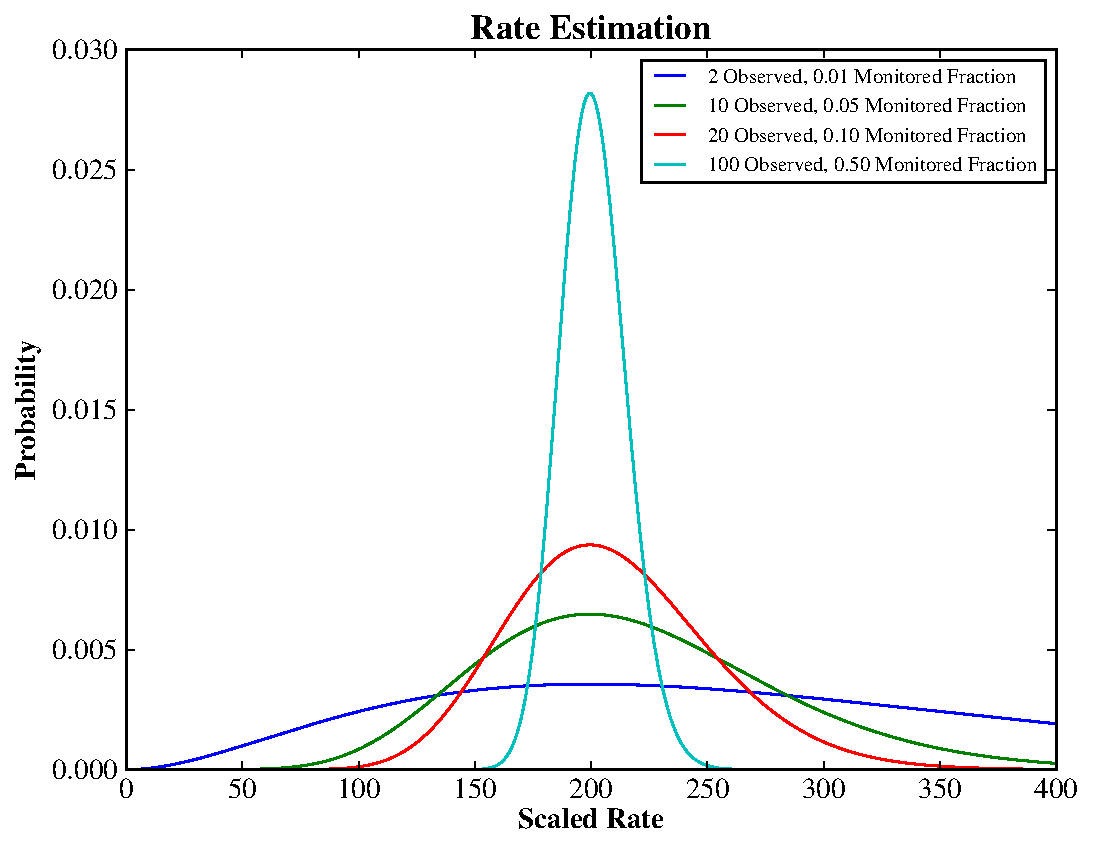
\includegraphics[width=\columnwidth]{./figures/rates.pdf}

\caption{\textbf{Example of rate estimation.} Spread of each distribution
shows the effect of the monitored fraction on rate certainty.}

\label{fig-rateexample}
\end{figure}

\subsection{Rate Estimation}
\label{subsec-rates}

When PocketParker receives arrival and departure event information, it knows
something concrete the state of the lot. However, to predict availability at
other times we need to adjust our estimation based on recently-observed
events, which we call rate estimation. To estimate the rate of events in the
entire population including hidden drivers, PocketParker must scale its rate
of parking events my monitored drivers appropriately. Next, we use these
scaled estimates to adjust the probability that a given lot has a certain
number of spots and has spots available.

During a time interval $t_0$ to $t_1$, PocketParker will observe some number
of searches $s_{obs}(t_0, t_1)$ or departures $d_{obs}(t_0, t_1)$ in any
given lot~\footnote{Without loss of generality our examples of scaling and
estimating rates use notation for the search rate.}. Note that the search
count includes both arrivals---successful searches---and implicit
unsuccessful searches derived from arrivals at related lots as explained
above. However, depending on the monitored fraction $f_m$ the true count
$s_{true}(t_0, t_1)$ is likely to be much larger. Rather than simply scaling
the count by $\frac{1}{f_m}$, we want to determine the probability
distribution over all possible true counts given the rate we observed and the
estimated monitored fraction as derived in Section~\ref{subsubsec-monitored}.
One reason we do not simply scale by $\frac{1}{f_m}$ is that intuitively our
uncertainty about the true count should be affected by $f_m$. If all drivers
use PocketParker, we know the true count exactly; if few do, we should be
uncertain about the true count.

To compute the probability distribution we treat $s_{obs}$ as the output of a
binomial distribution with probability $f_m$ and vary the number of trials.
Specifically:
%
\begin{equation} P(s_{true}; s_{obs}) = C \cdot {s_{obs} \choose s_{true}}
f_m^{(s_{obs})} \cdot (1 - f_m)^{(s_{true} - s_{obs})} \end{equation}
%
where $C$ is a renormalization constant equal to $\sum_{s_{true}} P$.
Figure~\ref{fig-rateexample} shows the resulting distribution for three
different values of $f_m$ with $s_{true} = 200$. While for all four values of
$f_m$, 200 is the most likely true count, as we desired the spread of the
distribution increases with decreasing $f_m$.

\subsubsection{Updating the count probabilities}

Given the probability that a lot has $n$ free spots at time $t_0$, $P_l(t_0,
n)$, we want to estimate the probabilities $P_l(t_1, n)$ at a later time
$t_1$. PocketParker uses recently-observed arrivals, implicit searches and
departures to estimate the search $s_{est}$ and departure $d_{est}$ rates the
lot experienced between $t_0$ and $t_1$. Currently, we use arrival and
departuress over a fixed-size window of time $I$ before $t_0$, $s_{obs}(t_0 -
I, t_0)$ scaled to the length of the interval $t_0$ to $t_1$:
%
\[s_{est}(t_0, t_1) = s_{obs}(t_0 - I, t_0) \cdot \frac{(t_1 - t_0)}{I} \]
%
The value of $s_{est}(t_0, t_1)$ is then scaled as described above to
determine the distribution of $s_{true}$. Intuitively, PocketParker currently
assumes the rates experienced over the last $I$ time interval will continue.
It may be possible to perform better rate estimation by using historical
information, but this is left as future work.

The distribution of search rates $s_{true}(t_0, t_1)$ represents the
probabilities that the number of available spots in the lot will decline,
whereas the departure rate $d_{true}(t_0, t_1)$ represents the probability
the number of spots will increase due to departures. The convolution of $-1
\cdot s_{true}$ and $d_{true}$, $\Delta(t_0, t_1)$, represents the change in
the number of spots produced by the specific combination of arrival and
departure rates. A further convolution of $\Delta(t_0, t_1)$ with $P_l(t_0,
n)$ produces $P_l(t_1, n)$, the desired probability at $t_1$:
%
\[ P_l(t_1, n) = P_l(t_0, n) * (-1 \cdot s_{true}(t_0, t_1) * d_{true}(t_0,
t_1)) \]
%
where $*$ represents the discrete convolution.

Note that the convolution of $P_l$ with $\Delta$ can cause non-zero
probabilities in $P_l$ that violate our boundary conditions, namely that
$P_l(n < 0) = 0$ and $P_l(n > C) = 0$ where $C$ is the estimated capacity of
the lot. To correct this, we simply set $P_l(n = 0) = \sum_{n < 0} P_l(n)$
and $P_l(n = C) = \sum_{n > C} P_l(n)$, assigning all the probability that
the lot has less that zero free spots to the zero state and all probability
that it has more than the capacity of the lot of free spots to the empty
state.

\subsubsection{Rateless spreading}

Intuitively, if the departure rate exceeds the arrival rate, the probability
mass of $\Delta$ will lie primarily to the positive side and it will shift
$P_l$ in the positive direction, producing higher probabilities that more
spots are available in the lot and lowering the probability that the lot is
full. The opposite is true when the search rate exceeds the arrival rate.

An important case is intervals during which PocketParker has observed neither
arrivals nor departures in a given lot. In this case, $\Delta$ will be
centered around $0$ but have a spread determined by the monitored fraction.
Its effect on $P_l$ will be to redistribute the probability mass more evenly
across the entire interval from $0$ to $C$. Taken over many intervals, the
probability of the lot having any number of spots available will equalize,
which is what we would expect: after a long period without any information,
all states become equally likely and we cannot make an accurate prediction of
the state of the lot. Note also that the speed at which the probabilities are
redistributed through rateless spreading is determined again by the monitored
fraction. The fewer drivers we monitor, the more quickly we lose all memory
of the state of the lot.

\begin{figure*}
  \centering
  \begin{subfigure}[b]{0.32\textwidth}
    \centering
    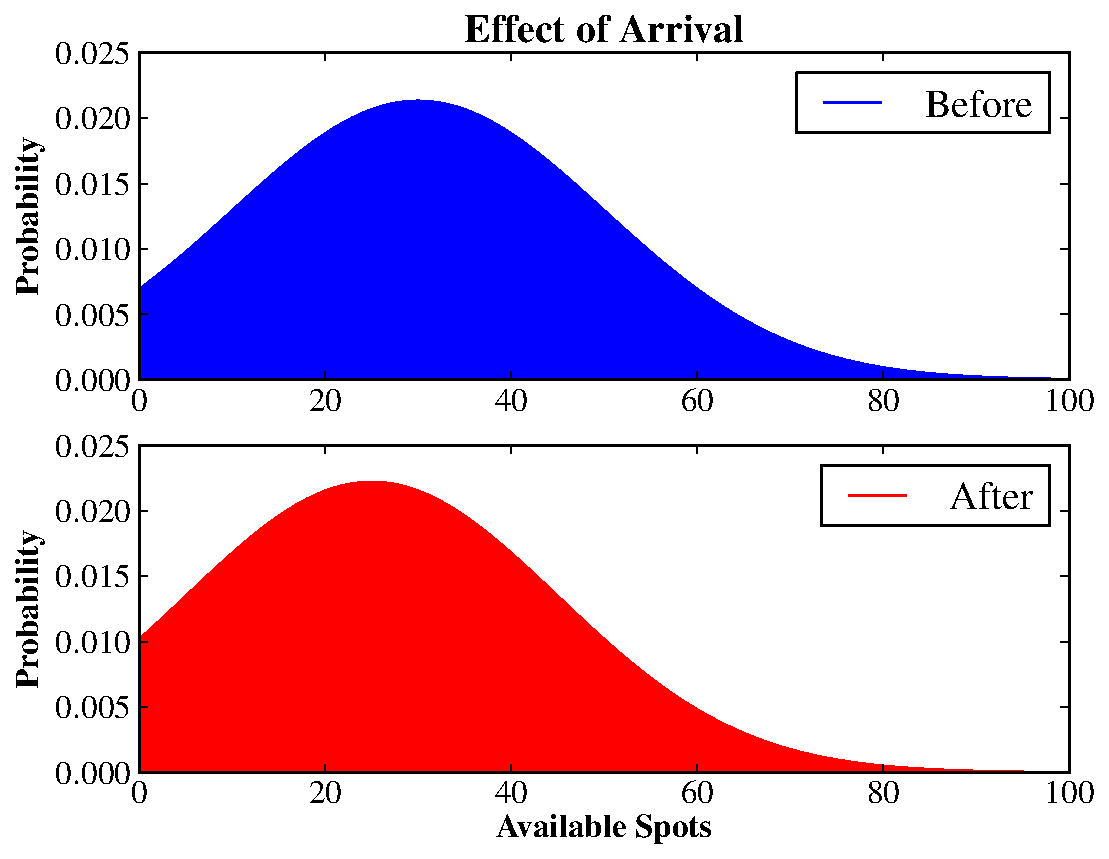
\includegraphics[width=\textwidth]{./figures/arrival.pdf}
    \caption{Effect of arrival.}
    \label{fig-examples-arrival}
  \end{subfigure}
  \begin{subfigure}[b]{0.32\textwidth}
    \centering
    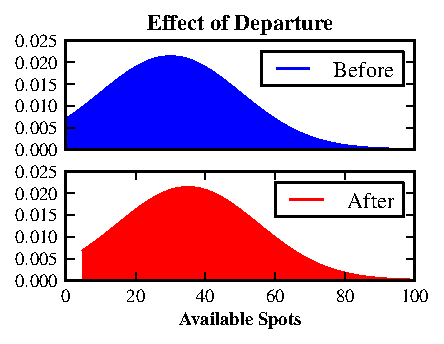
\includegraphics[width=\textwidth]{./figures/departure.pdf}
    \caption{Effect of departure.}
    \label{fig-examples-departure}
  \end{subfigure}
  \begin{subfigure}[b]{0.32\textwidth}
    \centering
    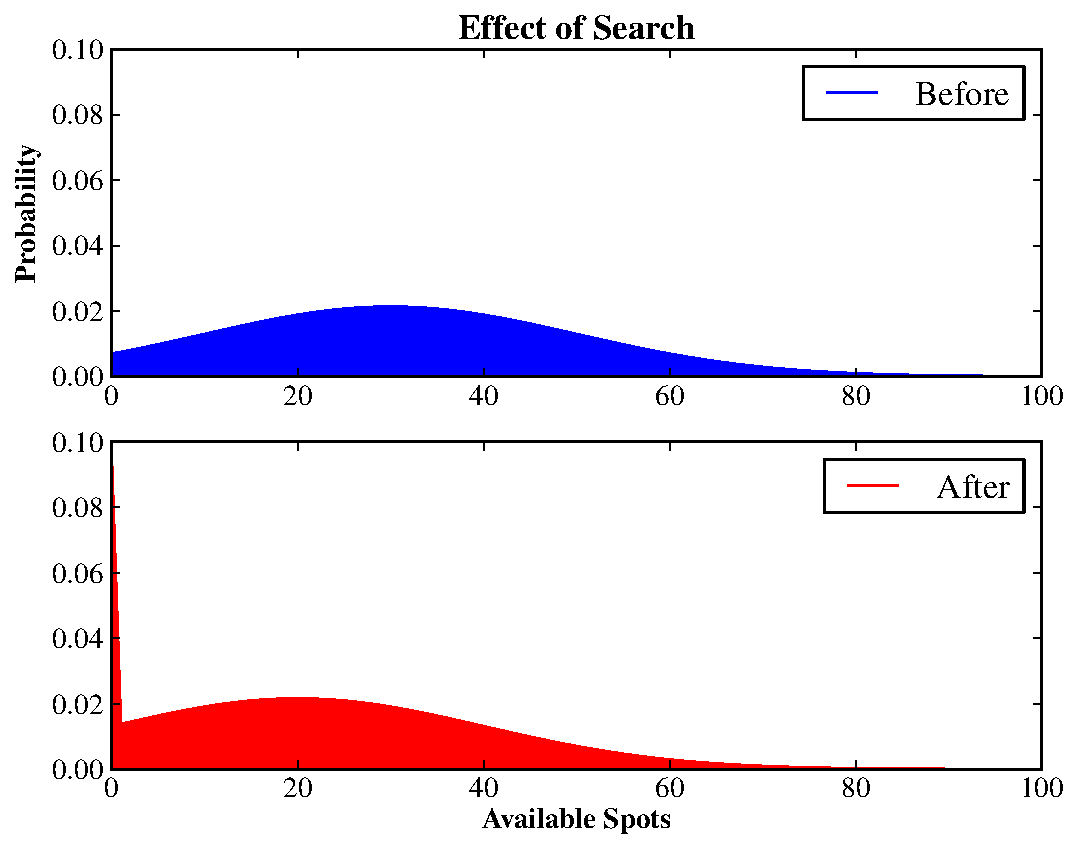
\includegraphics[width=\textwidth]{./figures/search.pdf}
    \caption{Effect of search.}
    \label{fig-examples-search}
  \end{subfigure}
  \caption{\textbf{Effect of different types of events on the lot availability
  distribution.} Arrivals, departures, and implicit searches each have a
  different instantaneous effect on PocketParker's availability distribution.}
  \label{fig-examples}
\end{figure*}

\subsection{Online Updates}
\label{subsec-online}

Finally, we conclude by describing how PocketParker uses arrival to adjust
its availability model instantaneously at runtime. Each arrival and departure
received represent strong positive information---moments when PocketParker
knows either that a spot just existed (arrival) or now exists (departure).
Unsuccessful implicit searches, in contrast, represent weaker negative
information, both because they were not have actually been observed by
PocketParker and so may not have actually taken place, or because they may
not have been thorough.

Departures produce an intuitive change to the probability distribution. When
a user departs, we know at that moment that there is a free spot in the lot,
so we can set $P_l(t, 0) = 0$ and renormalize the distribution. Arrivals
provide two somewhat conflict pieces of information. First, PocketParker
knows that at the time of the arrival there was a spot free, so in this way
arrivals indicate that the lot is not full. However, PocketParker also knows
that immediately after an arrival the lot has one fewer available spots. So
we incorporate arrivals in two steps. First, we set $P_l(t, 0) = 0$
indicating the availability of a spot and renormalize the distribution.
Second, we shift the entire distribution downward by one spot, $P_l(t, n) =
P_l(t, n - 1)$, reflecting the loss of a spot.

\subsubsection{Weighted arrivals and departures}

This is the most conservative approach representing what we definitely know.
However, if we assume that our monitored drivers are representative of some
larger number of hidden drivers, we may set $P_l(t, n < X) = 0$ for some $X$
larger than 1 and scaling with $\frac{1}{f_m}$. For our experiments we choose
the conservative approach and set $X = 1$. We discuss in
Section~\ref{sec-future} how users may customize the behavior of PocketParker
to be more or less aggressive in locating parking spots, trading off time for
a potentially more desirable spot.
